For the main control of the system, a State Machine with singleton pattern design is used. Every state is designed to be as small as possible. For the German Open 2015, we implemented three main states divided on smaller sub-states: move, grasp and deliver (see figure~\ref{fig:SM}).

On the initialization state, the robot receives the map and localizes itself on it. A state Idle is entered after that which waits until a task is received from the referee box. The complete task is divided into smaller subtasks and managed in stateNext. 

The first step is always driving to a specific position with a specific orientation. In this case, the path planner estimates a trajectory on the map. The robot drives to the desired position by following the calculated waypoints. Once the moving task is finished the state machine returns to StateNext, to process the next task.

In case of grasping, the robot approaches the service area and the state machine enters stateFindDesiredObject. After localizing this object, it is grasped and stored on the back of the robot.

%If we want to grasp an object, we would first smoothly approach to the service area and go to stateFindDesiredObject. After localizing the position of the desired object, we grasp it, lay it in our back and return back from the service area. 

In case of delivering an object, the robot also moves into the service arena, picks the object from its back and delivers it to the service arena.

%we also approach smoothly to the service area but this time we will pick up the object from our back and deliver it on the service area. Finally we return back from the service area and go again to StateNext.

The State Machine framework can be found on GitHub under our Laboratory’s repository: ”autonohm/obviously”.

\begin{figure}[htbp]
	\centering
	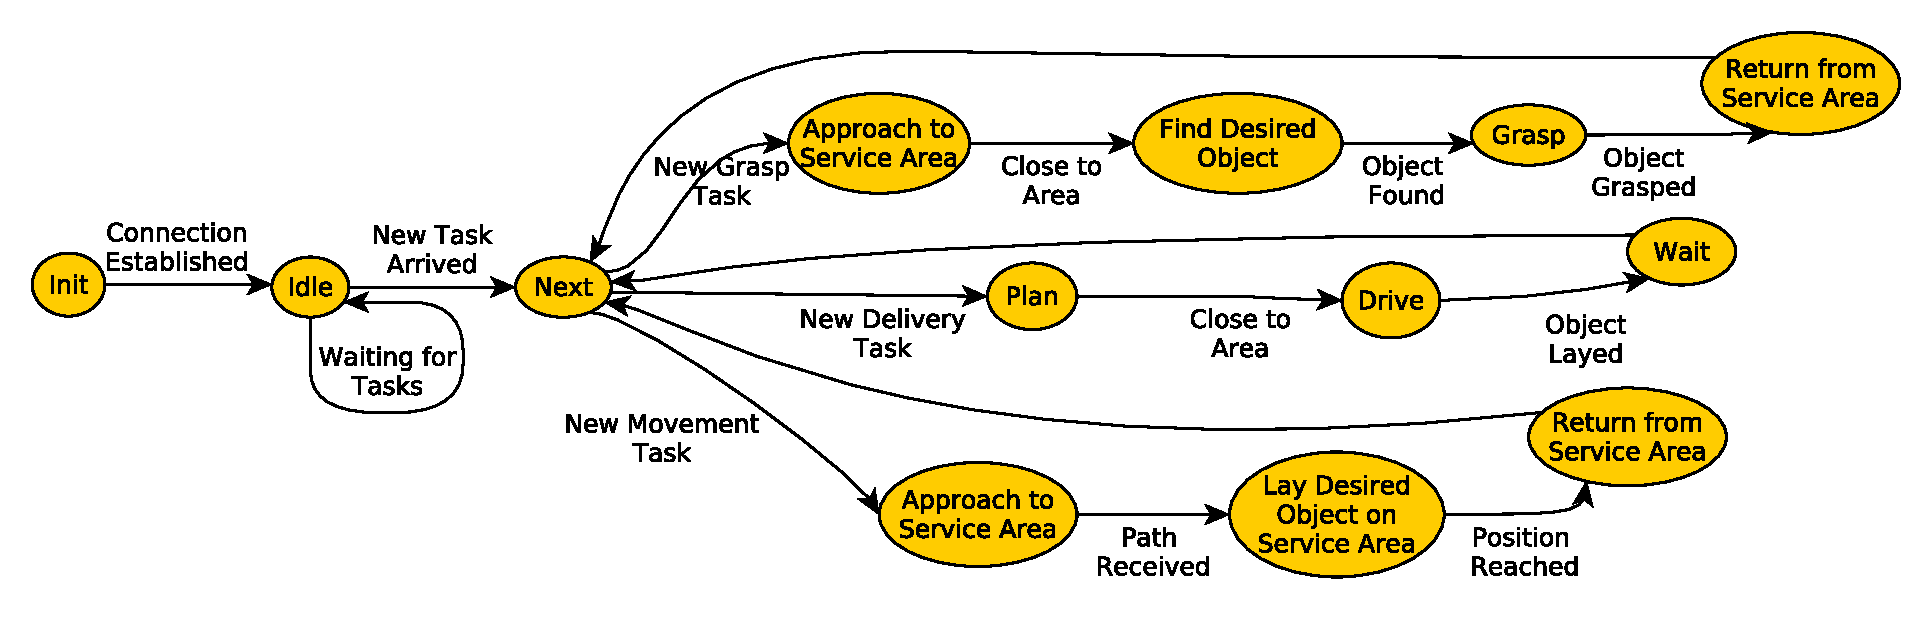
\includegraphics[width=\textwidth]{img/sm}
	\caption{Structure of the Statemachine}
	\label{fig:SM}
\end{figure}